\documentclass[letterpaper,11pt]{article}

\usepackage{graphicx}
\usepackage{multicol}
\usepackage{fullpage}
\usepackage{csquotes}
\usepackage[margin=0.75in,letterpaper]{geometry}
\setlength{\footskip}{15pt}
\setlength{\belowcaptionskip}{9pt}
\usepackage{censor}
\usepackage{floatflt}
\usepackage{xspace}
\usepackage[margin=1cm,skip=9pt]{caption}
\usepackage{ulem}
\usepackage{tikz}
\usetikzlibrary{shadows}

% https://tex.stackexchange.com/questions/5226/keyboard-font-for-latex
\newcommand*\keys[1]{%
  \tikz[baseline=(key.base)]
    \node[%
      draw,
      fill=white,
      drop shadow={shadow xshift=0.25ex,shadow yshift=-0.25ex,fill=black,opacity=0.75},
      rectangle,
      rounded corners=2pt,
      inner sep=1pt,
      line width=0.5pt,
      minimum width=1.1em,
      font=\scriptsize\sffamily
    ](key) {#1\strut}
  ;
}

\linespread{0.95}
\def\degC{$^{\circ}$C }
\def\degf{$^{\circ}$F }
\def\vol #1 {{\bf #1}, $\;\;$}
\def\refer{\par\noindent\hangindent\parindent\hangafter1}


\title{\vspace{-2.0cm}Herzmann Family Christmas Letter 2021}
\author{Daryl Herzmann${}^1$, Elizabeth Herzmann${}^2$, Margaret 
Herzmann${}^3$,\\
Robert Herzmann${}^3$, AND Charlotte Herzmann${}^4$ \\
\textit{${}^1$Vaxed + Horse Dewormer}`d,
\it{${}^2$Fully Vaxed + Booster},
\it{${}^3$Fully Vaxed},
\it{${}^4$Full of Bologna}}
\date{12 December 2021}

\makeatletter
\newenvironment{tablehere}
  {\def\@captype{table}}
  {}

\newenvironment{figurehere}
  {\def\@captype{figure}}
  {}
\makeatother

\newcommand{\Line}[0]{%
  \rule{0cm}{0cm}\\\hrule\rule{0cm}{0cm}%
}

%\addtolength{\textheight}{1.5in}

\begin{document}
\maketitle
\vspace{-0.75cm}
\begin{abstract}
We all survived the year, so you will find a proper accounting of our various
activities along with a tasteful level of snark.
\end{abstract}

\vspace{-0.5cm}

\noindent\makebox[\linewidth]{\rule{\textwidth}{1pt}}

\begin{multicols}{2}

\section{Introduction} 

As prescribed, our family size remains constant and comprises Daryl
\enquote{Daryl} (43), Elizabeth \enquote{Liz} (\blackout{28+}),
Margaret \enquote{Maggie Moo} (8), Robert \enquote{Bob-bert} (7), Charlotte
 \enquote{Charly Friend} (4), and one cat with a dog's name of Snoopy (13)
whose main purpose in life is to cause trouble.
   
\subsection{Housing and Domestics}

Our summer and winter dwelling remains the same physical structure with this
coming spring completing the tenth year of occupancy.  We had no remodeling projects
for the year and no significant damage from indiscretions made by the children
or tool-wielding father.  And as of this writing, Charlotte now has a lofted
bed, so all children now have the opportunity to fall from a 2$m$ height
each night.  Liz received an Insta-Pot for Christmas last year and it has
been a gift that keeps on giving.

\subsection{Conveyances}

No changes here, although Liz continues to scheme replacing her aging
and unexciting minivan with a Ford F-150 Lightning truck.  Any generous donations to the
Herzmann family for this worthy cause would be greatly appreciated.

\bigskip

\subsection{Employment}

Daryl is back to commuting to Iowa State University and writing buggy
software each day.  His highlights of the year include seeing 80 amps of
his power distribution equipment under flooded water and an artificial
intelligence (AI) system called Github CoPilot that now writes code for him
based on magic.  In fact, this system is writing this letter now and is
now suggesting to write. "This is a great example of how the computer
can be used to help people."

Liz still teaches at a middle school here in Ankeny.  The pandemic continues
to create a challenging environment with ever shifting policies and regulations.
Outside of that, teaching class at church, taking care of the kids, and keeping
the husband in-line consumes any remaining free time / energy Liz has.

The children remain unemployed, with plenty of free time and energy.

\section{Miss Charlotte}

Charlotte turns five in a few days and was concerned about not having much to
report on for this letter. So she recently deposited one of daddy's coins in her
belly bank (Figure 1) and remitted it a number of days later, without interest, by flushing it
down the toilet.  She will start Kindergarten next year and has committed to
finishing the thirteen years of schooling on time (Figure 2).

\begin{figurehere}
    \centering   
    \resizebox{.95\columnwidth}{!}{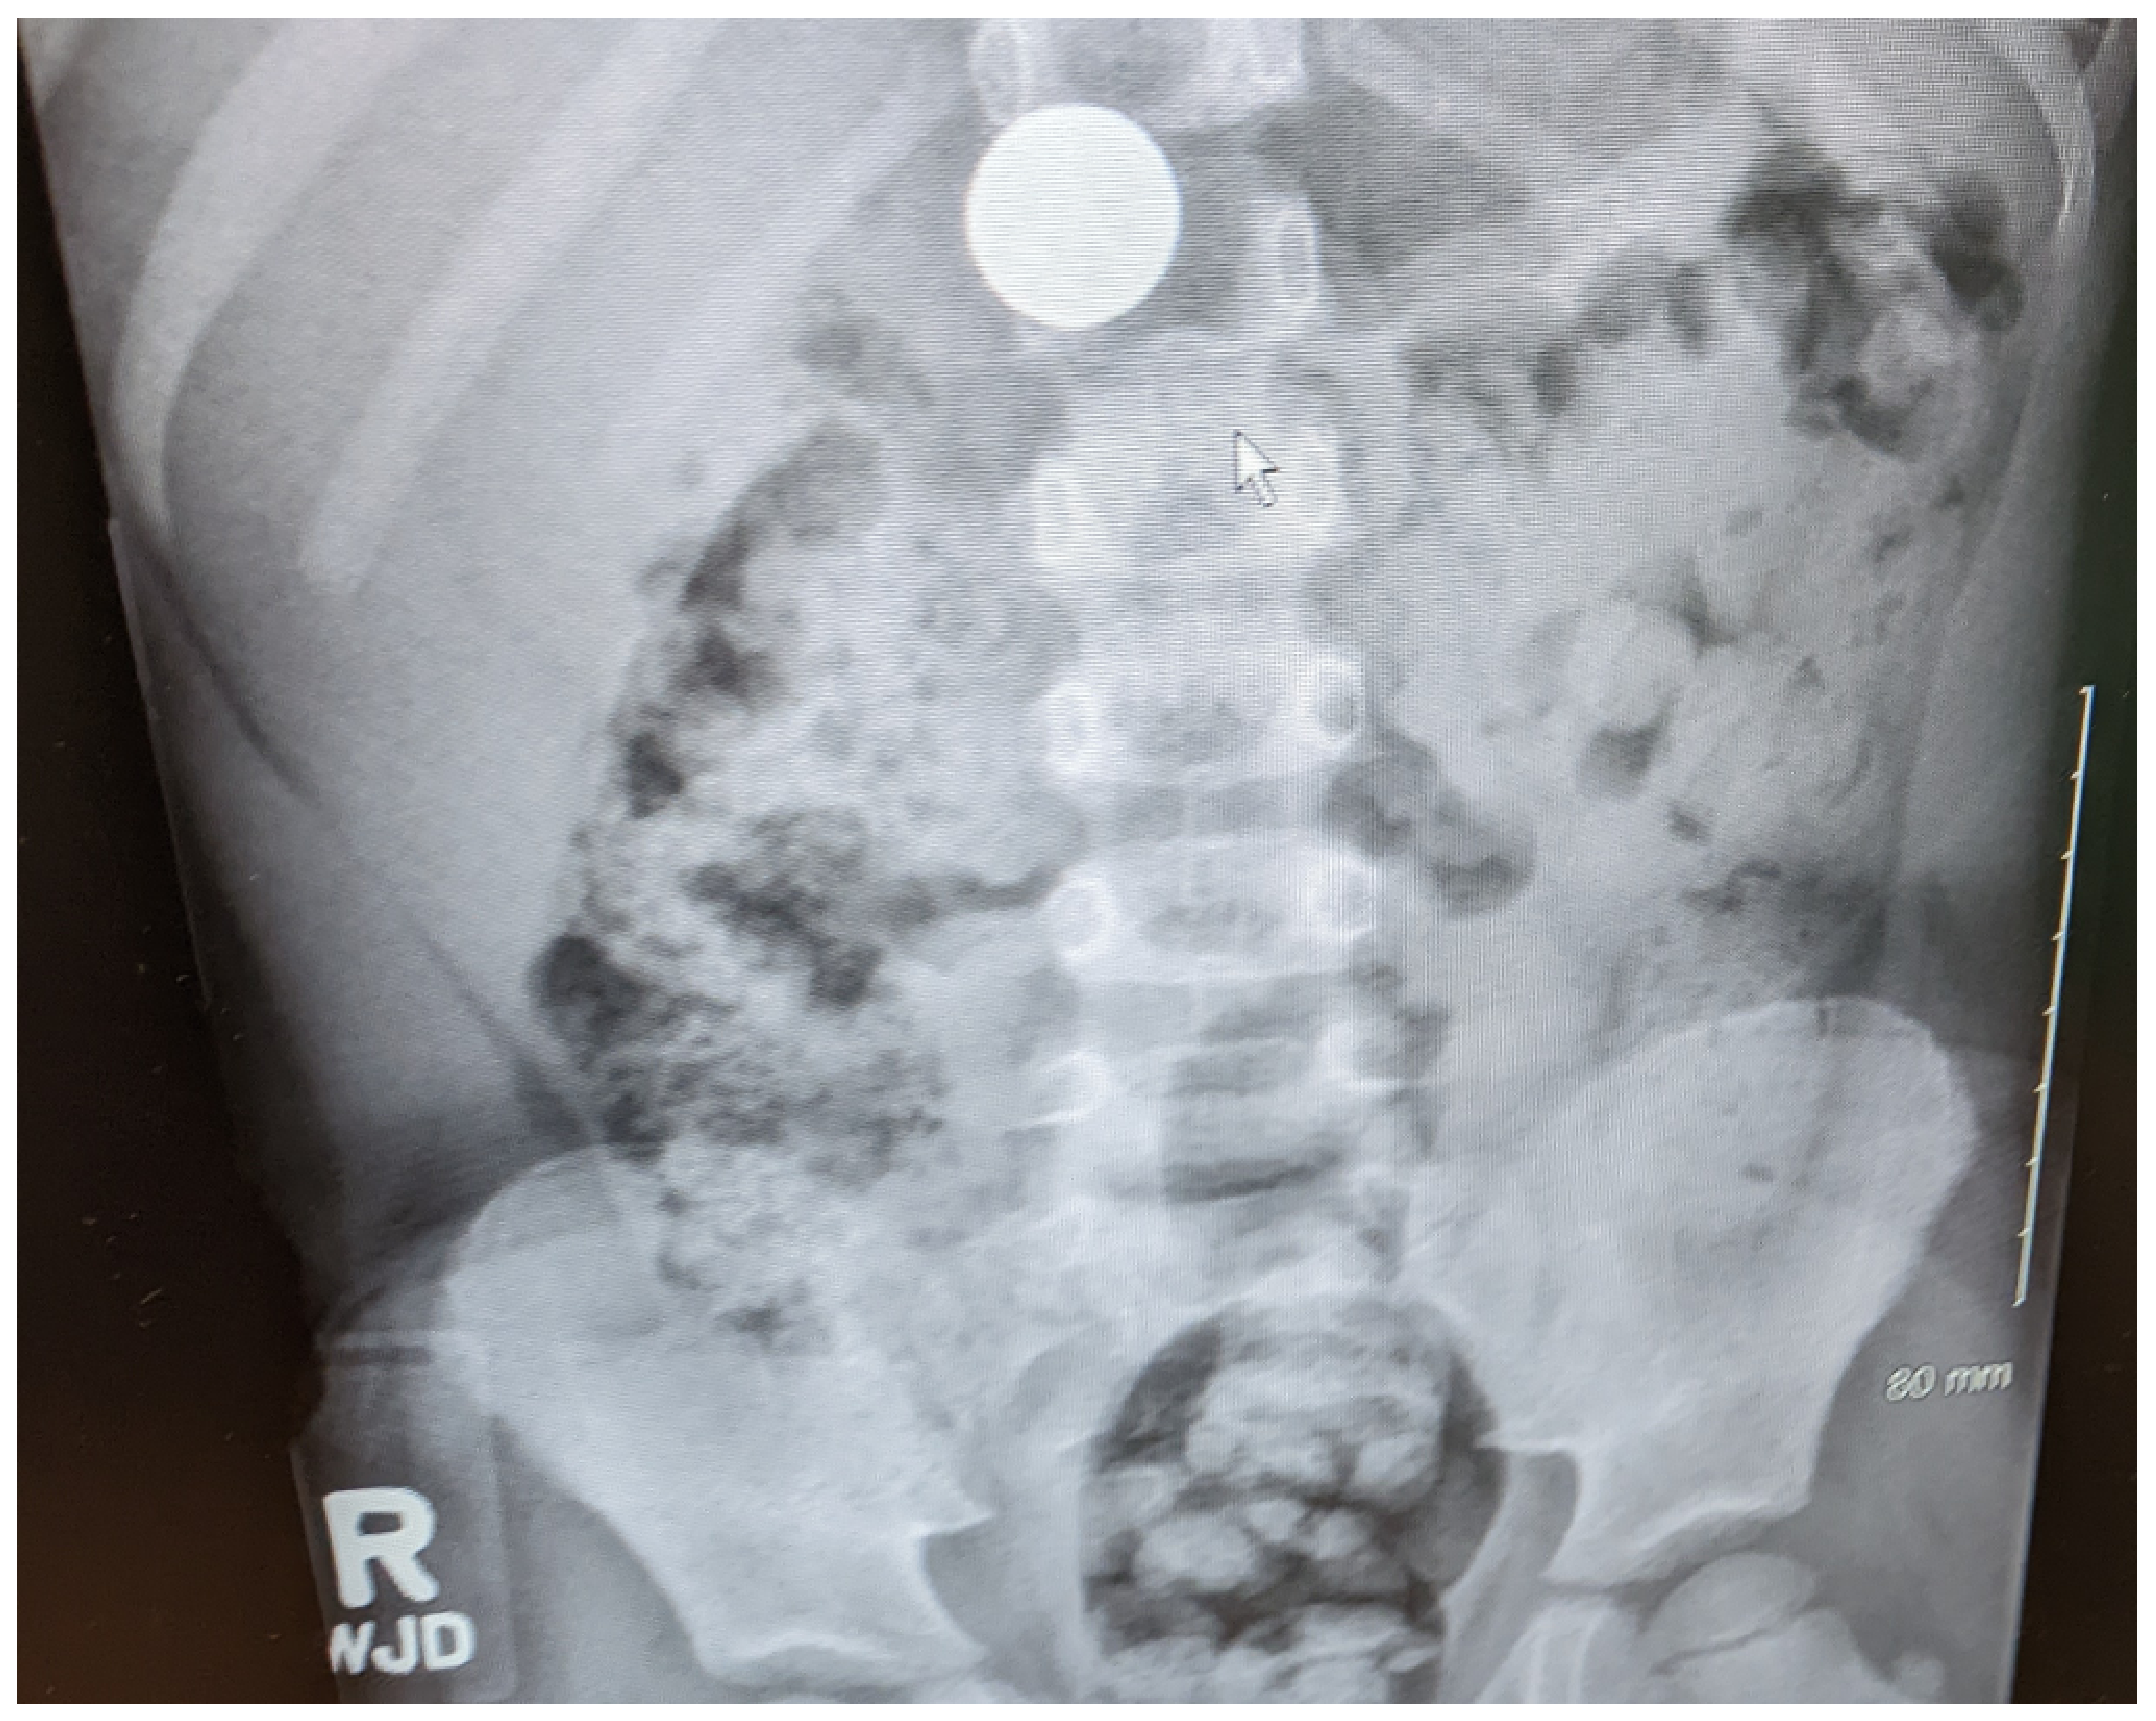
\includegraphics[angle=0]{plots/2021_f1.eps}}
    \caption{X-ray examination to determine how much money Charlotte owes in restitution.}
\end{figurehere}

\section{Mr Robert}

Robert continues to march to the beat of his own drum. He likes spending time
outside with as little clothing as possible.  He is making an honest effort to
learn the piano along with his sister.  He thoroughly enjoys the few days
we spend each fall at Grandma's farm helping her neighbors harvest corn. He
loves watching football and after determining which team the room is cheering for,
will vociferously support the other team.



\section{Miss Maggie}

Maggie is in ${3}^{rd}$ grade and still only completes one grade per year
(Figure 2). She would
like to provide you an itemized list of her activities:
\begin{itemize}
\item Near Easter, she had her first communion.
\item A few weeks ago, she danced in the \textbf{Nutcracker} with her dance studio.
\item She started piano lessons a few months ago and enjoys it.
\item She discovered the joy of eating kohlrabi.
\item She likes art.
\end{itemize}
``That's enough for now."

\begin{figurehere}
    \centering   
    \resizebox{.95\columnwidth}{!}{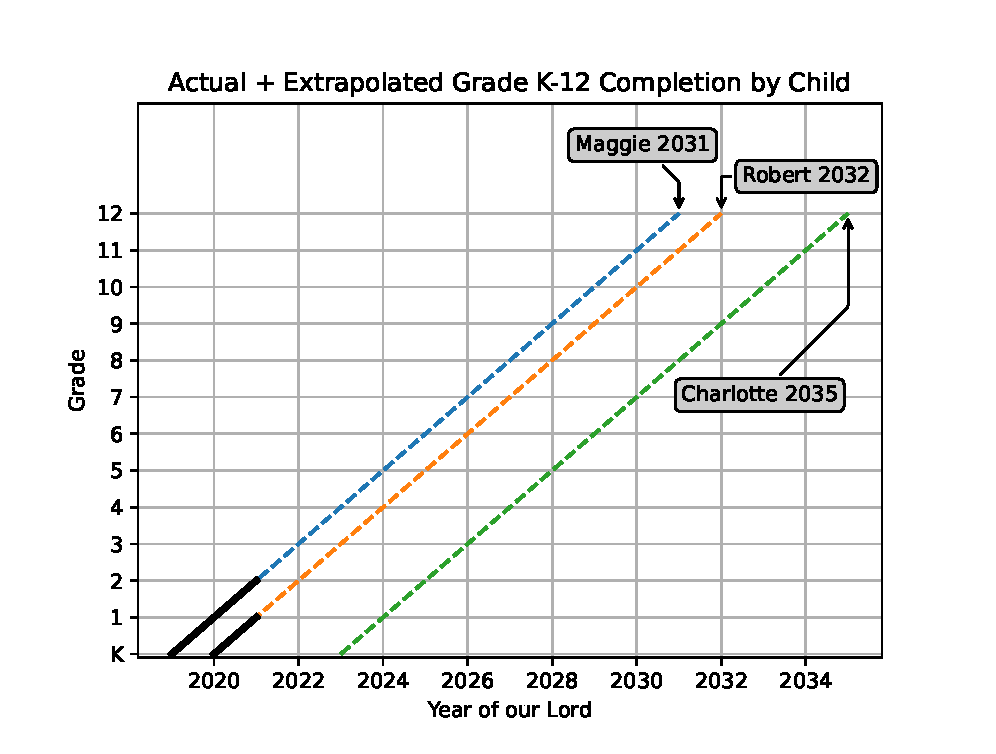
\includegraphics[angle=0]{plots/education.eps}}
    \caption{Observed and expected grade completion progress by child.}
\end{figurehere}


\section{Jamaica Galavanting}

To celebrate our \sout{10} ${11}^{th}$ wedding anniversary, we took a trip to the only
available hotel (\textit{cough}) in Jamaica, which unfortunately did not
permit children (\textit{cough, cough}), so the
kids had to stay home with the grandparents (\textit{cough, cough, cough}).
Herzmann et al (2020) promised that the obligatory swimsuit photo would be
included within this year's discourse.  Figure 3 is the highest
resolution photo we could find (\textit{more coughing}). For much of the trip,
Daryl repeated \textit{The Simpson's} quote, "It smells like
Otto's jacket" (Simpson, 1996). A forever-memory was sending a good friend a
postcard from there on 22 June and having it delivered in the states
on 22 November.

\begin{figurehere}
    \centering   
    \resizebox{.1\columnwidth}{!}{
\includegraphics[angle=0]{plots/f3_2021.eps}}
    \caption{Daryl and Liz, happily in love and such.}
\end{figurehere}

\section{Duluth Trip}

Parental guilt of not taking the kids to Jamaica led to a family trip to Duluth, MN.
We had a great time, but the kids were most interested in the nice pool,
with a slide, that the hotel had.  They all want to go back again,
so to experience the pool.  They also enjoyed watching the ships come in, the
lift bridge, Split Rock Lighthouse, and other sights sponsored here by
Visit Duluth (https://visitduluth.com).

\bigskip

\emph{Acknowledgments} Our family wishes to thank you for the generous 
support, prayers, cards, gifts, and \sout{visits} you have provided us in the past
year. Thanks to the non-color X-ray image included, we were able to avoid color
page costs this year. Please note that the format chosen for this
correspondence was completely Daryl's idea and execution. Full \LaTeX\xspace source can be found on Daryl's Github
page. 

\section{References}

\refer Github, 2021: https://github.com/akrherz/me , visited 12 Dec 2021.
\refer Herzmann, Daryl E., et al. Herzmann Family Christmas Letter, 2020.
\refer Simpson, Maggie. \textit{Homerpalooza}. The Simpsons; S7E24, 1996.

\end{multicols}

\end{document}
